\documentclass{article}

\usepackage{amssymb}
\setcounter{tocdepth}{3}
\usepackage{graphicx}
\usepackage{listings}
\usepackage{subfigure}
\usepackage{wrapfig}
\usepackage[hyperindex=false,colorlinks=false]{hyperref}
\usepackage{fullpage}

\begin{document}

\title{A Protocol for the Integration of Invasive Resource Management into Standard Batch Schedulers}
\author{Nishanth Nagendra}

\maketitle

\begin{abstract}
Invasive computing is a novel paradigm for the design and resource-aware programming of future parallel computing systems. It enables the programmer to write resource aware programs and the goal is to optimize the program for the available resources. Traditionally, parallel applications implemented using MPI are executed with a fixed number of MPI processes before submitting to a HPC(High Performance Computing) system. This results in a fixed allocation of resources for the job. Newer techniques in scientific computing such as AMR(Adaptive mesh refinement) result in applications exhibiting complex behavior where their resource requirements change during execution. Invasive MPI which is a part of an ongoing research effort to provide MPI extensions for the development of Invasive MPI applications will result in evolving jobs for the HPC systems at runtime supporting such AMR techniques. Unfortunately, using only static allocations result in the evolving applications being forced to execute using their maximum resource requirements that may lead to an inefficient resource utilisation. In order to support such parallel evolving applications at HPC centers there is an urgent need to investigate and implement extensions to existing resource management systems or develop an entirely new one. These supporting infrastructures must be able to handle the new kind of evolving jobs and the legacy rigid jobs intelligently and hence newer protocols for integration of such invasive resource management need to be now explored for integration into existing standard batch systems.
\end{abstract}


\section{Introduction}
Invasive computing is a novel paradigm for the design and resource-aware programming of future parallel computing systems. It enables the programmer to write efficient resource aware programs. This approach can be used to allocate, execute on and free resources during execution of the program. HPC infrastructure like Clusters, Supercomputers execute a vast variety of jobs, majority of which are parallel applications. These centers use intelligent resource management systems that should not only perform tasks of job management, resource management and scheduling but also satisfy important metrics like higher system utilization, job throughput and responsiveness. Traditionally, MPI applications are executed with a fixed number of MPI processes but with Invasive MPI they can evolve dynamically at runtime in the number of their MPI processes. This in turn supports advanced techniques like AMR where the working set size of applications change at runtime. These advancements entail an immediate need for stronger and intelligent resource management systems that can provide efficient resource utilization at HPC centers. They should also now be able to achieve much higher system utilisation, energy efficiency etc. compared to their predecessors due to elasticity of the applications.\par 
\noindent
\\Under the collaborative research project funded by the German research foundation(DFG) in the Transregional Collaborative Research Centre 89(TRR89), research efforts are being made to investigate Invasive computing approach vertically at different levels of abstraction right from the hardware up to the programming model. Invasive MPI is one such effort towards invasive programming with MPI where the application programmer has MPI extensions available using which he/she can specify at certain safe points in the program to allow for elasticity which means the application can evolve.
 
\subsection{Resource Management}
In order to support such parallel evolving applications at HPC centers there is an urgent need to investigate and implement extensions to existing resource management systems or develop an entirely new one. These supporting infrastructures must be able to handle the new kind of evolving jobs/applications and the legacy rigid jobs intelligently keeping in mind that they should now be able to achieve much higher system utilisation, energy efficiency etc compared to their predecessors due to the elasticity of the applications. Two of the most widely used resource managers on HPC systems are SLURM and TORQUE. The 2 major components in general of any sophisticated resource manager are the batch scheduler and the process manager.

\subsection{Batch Scheduling}
The batch scheduler accepts job descriptions given by end users some of which mention as to how long the job would run and the amount of resources it will need. It maintains a queue of jobs and dispatches them to the process manager based on some criteria and algorithms. The decisions made depend on the state of resources and also others like job priorities, fairness, waiting times etc. The process manager on the other hand has lesser intelligence and does the task of mapping the processes of a parallel application on the hardware based on the node list provided to it by the batch scheduler. In the context of invasive computing we need to be investigate for new requirements in the interaction between the batch scheduler and process manager. The decisions made by the batch scheduler need to be influenced to support evolving jobs.\par
\noindent
\\In contrast to the earlier uni-directional communication from batch scheduler to process manager, we now need to support a bi-directional communication between the two. The capabilities of existing batch schedulers could be leveraged rather than having to replace an entire system with a new one. The possiblity of supporting a new interface for the existing batch scheduler needs to be explored such that it communicates with a new invasive process management that controls a dedicated partition to support invasive computing. An investigation needs to be done on whether the existing interface of batch schedulers towards process manager could be extended or re-used and also on the possiblity of receiving feedback from the invasive process manager to allow the batch scheduler to be influenced. The invasive process manager one level below in the hierarchy as shown in the figure below will work on local metrics of the dedicated invasive partition within the cluster allocated by the batch scheduler.\par
\noindent
\\The investigations of this guided research are an initial study that will support the continuing research effort for developing Invasive MPI and extended resource management systems to support Invasive computing systems.

\begin{figure}[h]
\centering
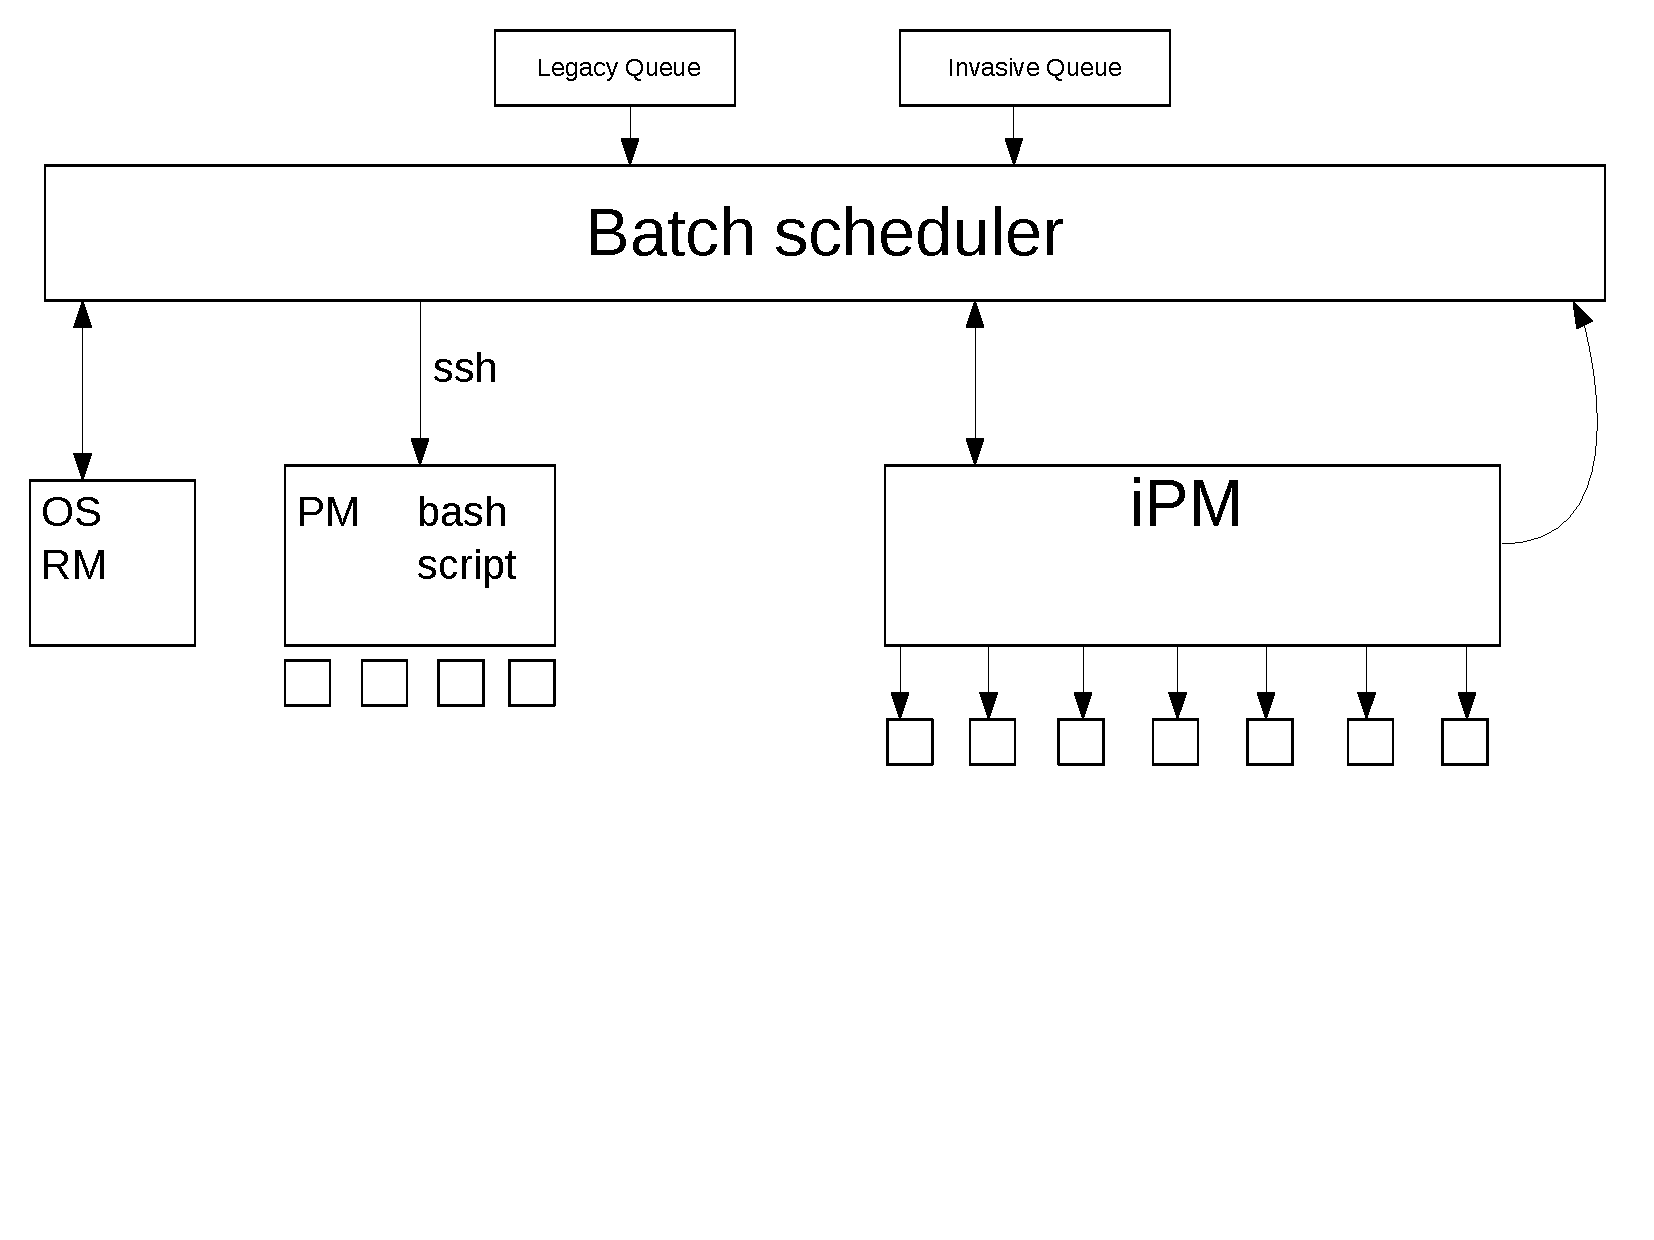
\includegraphics[width=0.65\textwidth, clip, trim=0mm 60mm 0mm 0mm]{data/architecture.pdf}
\vspace{-0.15in}
\caption{Invasive resource management architecture}
\label{fig:arch}
\end{figure}

\end{document}
